\documentclass[__main__.tex]{subfiles}
\begin{document}

\qtitle{С}{07}
Вычислите ёмкость сферического конденсатора, представленного двумя концентрическими обкладками, радиусы которых $r_1$ и $r_2$, диэлектрическая проницаемость вещества, заполняющего пространство между ними $\varepsilon$.\\

\textbf{Решение}\\
\begin{figure}[h]
    \center{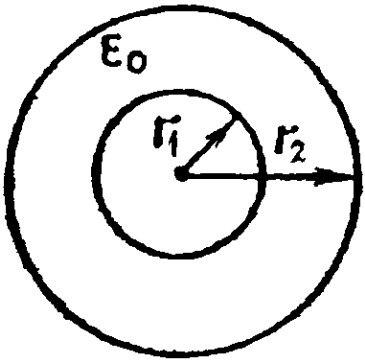
\includegraphics[width=0.2\linewidth]{c-07-1}}
\end{figure}

\textbf{Анализ}
\begin{enumerate}
    \item Поле обладает центральной симметрией. Решение целесообразно проводить в сферической системе координат, начало которой совмещено с центром шара.
    \item В этом случае вектор напряженности $\vec{E}$ имеет в любой точке, лежащей на сфере радиуса $r$  единственную радиальную составляющую $\vec{E} = E\cdot \vec{e}_r$
    \item В любой точке поверхности постоянного радиуса значения вектор $\vec{E}$ постоянен.
\end{enumerate}
\textbf{Аналитическое описание поля сферического конденсатора}
\begin{figure}[h]
    \center{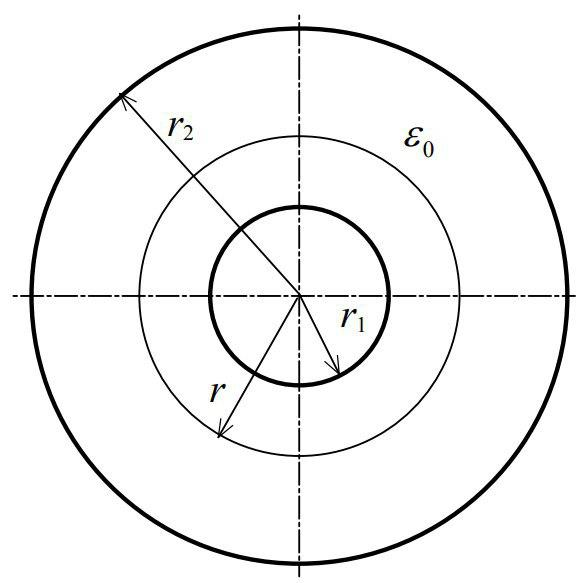
\includegraphics[width=0.4\linewidth]{c-07-2}}
\end{figure}

\begin{enumerate}
    \item По теореме Гаусса
          \begin{gather*}
              \oint_S\vec{E}d\vec{S} = \oint_SEdS = E\oint_SdS = E\cdot 4\pi r^2 = \frac{q}{\varepsilon_r \varepsilon_0}
          \end{gather*}
          где $q$ - заряд в области шара $r \leq r_2$ (заряд сферического конденсатора), $\varepsilon_r$ - относительная диэлектрическая проницаемость диэлектрика конденсатора, $\varepsilon_0 = 8.85\times 10^{-12}$ - диэлектрическая постоянная\\
          В итоге получаем
          \begin{gather*}
              E(r) = \frac{q}{4\pi \varepsilon_0 \varepsilon_r r^2}
          \end{gather*}
          Потенциал области
          \begin{gather*}
              \varphi = -\int\vec{E}d\vec{r}+c = -\int Edr +c = -\int \frac{q}{4\pi \varepsilon_0 \varepsilon_r r^2} dr +c = \frac{q}{4\pi \varepsilon_0 \varepsilon_r r}+c
          \end{gather*}
          Определим постоянную интегрирования $c$. Считая, что при $r\to\infty,\varphi\to 0$, получим $c = 0$:
          \begin{gather*}
              \varphi (r) = \frac{q}{4\pi \varepsilon_0 \varepsilon_r r}
          \end{gather*}
    \item Напряжение между обкладками конденсатора
          \begin{gather*}
              U = \varphi (r_1) - \varphi (r_2) = \frac{q}{4\pi \varepsilon_0 \varepsilon_r r_1} - \frac{q}{4\pi \varepsilon_0 \varepsilon_r r_2} = \frac{q}{4\pi \varepsilon_0 \varepsilon_r}\left(\frac{1}{r_1}-\frac{1}{r_2}\right)
          \end{gather*}
    \item Электроемкость конденсатора дается выражением
          \begin{gather*}
              C = \frac{q}{U} = \frac{q}{\frac{q}{4\pi \varepsilon_0 \varepsilon_r}\left(\frac{1}{r_1}-\frac{1}{r_2}\right)} = \frac{4\pi \varepsilon_0 \varepsilon_r r_1 r_2}{r_2-r_1}
          \end{gather*}
\end{enumerate}

\end{document}